\documentclass[11pt,a4paper]{article}

% ── Packages ──────────────────────────────────────────────────────────────────
\usepackage[margin=2.2cm]{geometry}
\usepackage[T1]{fontenc}
\usepackage[utf8]{inputenc}
\usepackage{lmodern}
\usepackage{microtype}
\usepackage{xcolor}
\usepackage{parskip}
\usepackage{titlesec}
\usepackage{booktabs}
\usepackage{array}
\usepackage{tabularx}
\usepackage{multirow}
\usepackage{graphicx}
\usepackage{amsmath}
\usepackage{amssymb}
\usepackage{enumitem}
\usepackage{fancyhdr}
\usepackage{pgfplots}
\usepackage{pgfplotstable}
\usepackage{tikz}
\usepackage{listings}
\usepackage{caption}
\usepackage{subcaption}
\usepackage{hyperref}

\pgfplotsset{compat=1.18}

% ── Colour palette ────────────────────────────────────────────────────────────
\definecolor{primary}{HTML}{1A3A5C}
\definecolor{accent}{HTML}{2980B9}
\definecolor{light}{HTML}{EAF4FB}
\definecolor{muted}{HTML}{7F8C8D}
\definecolor{gold}{HTML}{D4AC0D}
\definecolor{codegreen}{HTML}{27AE60}
\definecolor{codebg}{HTML}{F4F6F7}
\definecolor{rulecolor}{HTML}{AED6F1}

% ── Page style ────────────────────────────────────────────────────────────────
\pagestyle{fancy}
\fancyhf{}
\fancyhead[L]{\small\color{muted}IDC 606 — Final Report}
\fancyhead[R]{\small\color{muted}Smoothed Particle Hydrodynamics}
\fancyfoot[C]{\small\color{muted}\thepage}
\renewcommand{\headrulewidth}{0.4pt}
\renewcommand{\headrule}{\hbox to\headwidth{\color{rulecolor}\leaders\hrule height\headrulewidth\hfill}}

% ── Section formatting ────────────────────────────────────────────────────────
\titleformat{\section}{\large\bfseries\color{primary}}{}{0em}{}[{\color{accent}\rule{\linewidth}{1pt}}]
\titleformat{\subsection}{\normalsize\bfseries\color{primary}}{}{0em}{}
\titlespacing{\section}{0pt}{14pt}{6pt}
\titlespacing{\subsection}{0pt}{10pt}{4pt}

% ── Listings style ────────────────────────────────────────────────────────────
\lstset{
  backgroundcolor=\color{codebg},
  basicstyle=\ttfamily\footnotesize,
  keywordstyle=\color{accent}\bfseries,
  commentstyle=\color{muted}\itshape,
  stringstyle=\color{codegreen},
  frame=single,
  framerule=0pt,
  rulecolor=\color{rulecolor},
  breaklines=true,
  numbers=left,
  numberstyle=\tiny\color{muted},
  xleftmargin=1.5em,
  framexleftmargin=1.5em,
  language=Python,
}

% ── Metric / highlight boxes (no tcolorbox needed) ───────────────────────────
\newcommand{\metricbox}[2][primary]{%
  \colorbox{#1!10}{\textcolor{#1}{\bfseries#2}}%
}

\newsavebox{\hlbox}
\newenvironment{highlight}[1][]{%
  \def\hltitle{#1}%
  \begin{lrbox}{\hlbox}%
  \begin{minipage}{\dimexpr\linewidth-16pt\relax}%
  \vspace{4pt}%
  \ifx\hltitle\@empty\else
    \noindent\colorbox{accent}{\color{white}\bfseries\strut\,\hltitle\,}\par\vspace{6pt}%
  \fi
}{%
  \vspace{4pt}%
  \end{minipage}%
  \end{lrbox}%
  \par\vspace{4pt}%
  \noindent\colorbox{light}{\usebox{\hlbox}}%
  \par\vspace{4pt}%
}

% ══════════════════════════════════════════════════════════════════════════════
\begin{document}

% ── Title block ───────────────────────────────────────────────────────────────
\begin{tikzpicture}[remember picture, overlay]
  \fill[primary] (current page.north west) rectangle
    ([yshift=-3.8cm]current page.north east);
\end{tikzpicture}

\vspace*{-1.8cm}
{\color{white}
  \begin{center}
    \textbf{\Large IDC 606 — High-Performance Computing}\\[4pt]
    {\LARGE\bfseries Smoothed Particle Hydrodynamics Simulation}\\[6pt]
    \hrule height 0.6pt
    \vspace{6pt}
    {\normalsize
      Pahal Patel \quad|\quad Pranav Agrawal \quad|\quad
      Sanskaar Srivastava \quad|\quad Tanish Singla}\\[3pt]
    {\small\color{rulecolor}
      \href{https://github.com/D3bug1t/IDC_606_SPH}
           {\texttt{github.com/D3bug1t/IDC\_606\_SPH}}
      \quad\textbullet\quad April 2026}
  \end{center}
}
\vspace{0.5cm}

% ── Key results summary bar ────────────────────────────────────────────────────
\begin{center}
\renewcommand{\arraystretch}{1.4}
\begin{tabular}{@{}lll@{}}
  \toprule
  \textbf{Metric} & \textbf{Value} & \textbf{Notes} \\
  \midrule
  GPU Speedup vs CPU baseline   & \textbf{1914$\times$}         & RTX 6000 Blackwell, $N\approx40$K \\
  Measured FLOPS rating          & \textbf{8.95\,TFLOPS}        & spreadsheet-verified, 500-step average \\
  Peak SM utilisation            & \textbf{83.5\,\%}            & fused density+pressure kernel, $N=500$K \\
  Maximum stable particle count  & \textbf{500\,000}            & fixed-timestep RK4 \\
  \bottomrule
\end{tabular}
\end{center}

\vspace{0.4cm}

% ── 1  Overview ───────────────────────────────────────────────────────────────
\section{Overview}

Smoothed Particle Hydrodynamics (SPH) is a mesh-free Lagrangian method for simulating fluid
dynamics. Originally developed for astrophysical simulations, it is now widely used for
dam-break problems, free-surface flows, and ocean engineering. Unlike mesh-based methods
(FVM/FEM), SPH tracks a set of discrete particles, each carrying physical quantities such as
mass, density, pressure, and velocity. Field quantities are interpolated using a kernel function,
making SPH naturally suited to problems with large deformations and moving boundaries.

This project implements a Weakly Compressible SPH (WCSPH) solver accelerated on GPU using
\textbf{NVIDIA Warp}, a Python-native framework that JIT-compiles Python kernel functions to
CUDA C++ at runtime. The canonical benchmark is the \textbf{2-D dam-break problem}: a column
of water initially at rest is released and propagates across a dry bed under gravity. The goal
is to achieve physically accurate results while maximising computational throughput through
algorithmic and GPU-level optimisations.

\vspace{6pt}
\begin{center}
\begin{tabular}{llc}
  \toprule
  \textbf{Parameter} & \textbf{Symbol} & \textbf{Value} \\
  \midrule
  Domain width              & $L_x$        & 20.0\,m \\
  Domain height             & $L_y$        & 15.0\,m \\
  Fluid density (rest)      & $\rho_0$     & 1000\,kg\,m$^{-3}$ \\
  Speed of sound            & $c_0$        & 20\,m\,s$^{-1}$ \\
  EOS exponent              & $\gamma$     & 7 \\
  Viscosity coefficient     & $\alpha$     & 1.0 \\
  Gravitational acceleration& $g$          & 9.81\,m\,s$^{-2}$ ($-y$) \\
  Particle spacing          & $\Delta x$   & 0.01\,m \\
  Smoothing length factor   & $h/\Delta x$ & 1.6 \\
  Timestep                  & $\Delta t$   & $1\times10^{-4}$\,s \\
  Simulation duration       & $T$          & 5.0\,s \\
  Total particles (500K run)& $N$          & 500\,000 \\
  \bottomrule
\end{tabular}
\end{center}

% ── 2  Executive Summary ──────────────────────────────────────────────────────
\section{Summary}

Starting from a naïve CPU baseline, we achieved a \textbf{1914$\times$ speedup}
by combining spatial hashing, JIT-compiled GPU kernels, device-resident arrays,
and a fused 4th-order Runge–Kutta integrator.

\vspace{4pt}
\begin{center}
\begin{tabular}{lcc}
  \toprule
  \textbf{Metric} & \textbf{CPU Baseline} & \textbf{GPU (Warp)} \\
  \midrule
  Runtime (5\,000 steps, $N{\approx}40\text{k}$) & 957\,s & 0.5\,s \\
  Integrator & Leapfrog & Fused RK4 \\
  Neighbour search & $O(N^2)$ & $O(N)$ HashGrid \\
  Measured FLOPS rating & — & 8.95\,TFLOPS \\
  SM throughput (fused kernel) & — & 83.5\,\% \\
  \bottomrule
\end{tabular}
\end{center}

% ── 2  Mathematical Formulation ───────────────────────────────────────────────
\section{Mathematical Formulation}

\subsection{SPH Kernel Interpolation}

In SPH, any field quantity $A$ at particle $i$ is approximated as a weighted sum over all
particles $j$ within the support radius $2h$:
\[
  A(\mathbf{r}_i) = \sum_j \frac{m_j}{\rho_j}\,A_j\,W(\mathbf{r}_i - \mathbf{r}_j,\,h)
\]
where $W$ is the kernel function, $h$ is the smoothing length, and $m_j/\rho_j$ is the volume
element of particle $j$.  The kernel must satisfy normalisation ($\int W\,\mathrm{d}\mathbf{r}=1$)
and approach a Dirac delta as $h\to 0$.

\subsection{Cubic Spline Kernel}

We use the 2-D Monaghan cubic spline kernel (M4), which offers $C^2$ continuity and compact
support radius $2h$:
\[
  W(q) = \frac{10}{7\pi h^2}
  \begin{cases}
    1 - \tfrac{3}{2}q^2 + \tfrac{3}{4}q^3 & 0 \le q < 1 \\[4pt]
    \tfrac{1}{4}(2-q)^3                    & 1 \le q < 2 \\[4pt]
    0                                       & q \ge 2
  \end{cases}
\]
where $q = r/h = |\mathbf{r}_i - \mathbf{r}_j|/h$.  The gradient used in force calculations is:
\[
  \nabla W = \frac{\mathrm{d}W}{\mathrm{d}q}\,\frac{1}{hr}\,(\mathbf{r}_i - \mathbf{r}_j),
  \qquad
  \frac{\mathrm{d}W}{\mathrm{d}q} = \frac{10}{7\pi h^2}
  \begin{cases}
    -3q + \tfrac{9}{4}q^2 & 0 \le q < 1 \\[4pt]
    -\tfrac{3}{4}(2-q)^2  & 1 \le q < 2
  \end{cases}
\]

\subsection{Density Estimation}

Particle density is computed by direct summation (the summation density approach), which
conserves mass by construction:
\[
  \rho_i = \sum_j m_j\,W(|\mathbf{r}_i - \mathbf{r}_j|,\,h)
\]
The per-particle cost is $O(k)$ where $k \approx 21$ is the mean neighbour count inside a
circle of radius $2h$ at typical packing $\Delta x = 0.01$\,m, $h = 0.016$\,m.

\subsection{Weakly Compressible Pressure — Tait EOS}

Instead of enforcing strict incompressibility (which would require solving a pressure Poisson
equation), WCSPH uses the Tait equation of state to relate density perturbations to pressure:
\[
  P_i = \frac{c_0^2 \rho_0}{\gamma}
        \left[\left(\frac{\rho_i}{\rho_0}\right)^{\!\gamma} - 1\right]
\]
With $c_0 = 20$\,m\,s$^{-1}$ and $\gamma = 7$ this gives a stiff spring restoring force that keeps
density fluctuations below $\sim$1\,\%.  The bulk modulus is $K = c_0^2\rho_0 = 4\times10^5$\,Pa.
The Mach number of the flow must remain below 0.1 for WCSPH to be accurate.

\subsection{Momentum Equation \& Artificial Viscosity}

The SPH momentum equation in symmetric form (conserving linear momentum exactly) is:
\[
  \frac{\mathrm{d}\mathbf{v}_i}{\mathrm{d}t}
  = -\sum_j m_j
    \left(\frac{P_i}{\rho_i^2} + \frac{P_j}{\rho_j^2} + \Pi_{ij}\right)
    \nabla_i W_{ij} + \mathbf{g}
\]
The Monaghan artificial viscosity $\Pi_{ij}$ damps spurious oscillations and prevents particle
interpenetration:
\[
  \Pi_{ij} =
  \begin{cases}
    \displaystyle -\frac{\alpha\,\bar{c}_{ij}\,\mu_{ij}}{\bar{\rho}_{ij}}
      & \mathbf{v}_{ij}\cdot\mathbf{r}_{ij} < 0 \text{ (approaching)} \\[6pt]
    0 & \text{otherwise}
  \end{cases}
  \qquad
  \mu_{ij} = \frac{h\,(\mathbf{v}_{ij}\cdot\mathbf{r}_{ij})}{|\mathbf{r}_{ij}|^2 + 0.01h^2}
\]
where $\bar{c}_{ij} = (c_i+c_j)/2$ is the mean sound speed and $\bar{\rho}_{ij}$ the mean
density.  The $0.01h^2$ term prevents singularity when particles are very close.

\subsection{Time Integration: Leapfrog vs.\ RK4}

Two integrators were implemented and benchmarked.

\textbf{Leapfrog (Velocity Verlet) : 2nd order, 1 force evaluation per step:}
\begin{align*}
  \mathbf{v}_i(t+\tfrac{\Delta t}{2}) &= \mathbf{v}_i(t) + \mathbf{a}_i(t)\,\tfrac{\Delta t}{2} \\
  \mathbf{r}_i(t+\Delta t)            &= \mathbf{r}_i(t) + \mathbf{v}_i(t+\tfrac{\Delta t}{2})\,\Delta t \\
  \mathbf{v}_i(t+\Delta t)            &= \mathbf{v}_i(t+\tfrac{\Delta t}{2}) + \mathbf{a}_i(t+\Delta t)\,\tfrac{\Delta t}{2}
\end{align*}

\textbf{Runge–Kutta 4 : 4th order, 4 force evaluations per step:}
\begin{align*}
  k_1 &= f(\mathbf{r},\,\mathbf{v},\,t) \\
  k_2 &= f\!\left(\mathbf{r}+k_1\tfrac{\Delta t}{2},\;\mathbf{v}+k_1\tfrac{\Delta t}{2},\;t+\tfrac{\Delta t}{2}\right) \\
  k_3 &= f\!\left(\mathbf{r}+k_2\tfrac{\Delta t}{2},\;\mathbf{v}+k_2\tfrac{\Delta t}{2},\;t+\tfrac{\Delta t}{2}\right) \\
  k_4 &= f\!\left(\mathbf{r}+k_3\Delta t,\;\mathbf{v}+k_3\Delta t,\;t+\Delta t\right) \\
  \mathbf{r}(t+\Delta t) &= \mathbf{r}(t) + \frac{\Delta t}{6}(k_1 + 2k_2 + 2k_3 + k_4)
\end{align*}

RK4 is $4\times$ more expensive per step but allows a larger stable $\Delta t$ and achieves
higher accuracy per unit of simulation time, making it the preferred method for production runs.

% ── 4  Algorithm: Hash Grid Neighbour Search ──────────────────────────────────
\section{Algorithm: Hash Grid Neighbour Search}

The dominant algorithmic optimisation is replacing the naïve $O(N^2)$ all-pairs search with an
$O(N)$ hash-grid-based search using \texttt{wp.HashGrid}. The domain is divided into a uniform
grid of cells of width $2h$. Each particle hashes its $(x,y)$ position into a cell index; only
the $3\times3 = 9$ adjacent cells need to be searched per query particle, giving $\sim$21
actual neighbours on average and reducing complexity from $O(N^2)$ to $O(N)$.

\vspace{4pt}
\begin{center}
\begin{tabular}{lll}
  \toprule
  \textbf{Search Method} & \textbf{Complexity} & \textbf{Time ($N$=50\,K, 100 steps)} \\
  \midrule
  All-pairs (naïve)          & $O(N^2)$ & ${\sim}1000$\,s \\
  Hash-grid neighbour search & $O(N)$   & ${\sim}3.5$\,s \\
  Speedup                    & —        & ${\sim}285\times$ \\
  \bottomrule
\end{tabular}
\end{center}

\subsection{Build Phase}

\lstset{language={}, mathescape=true, numbers=none, frame=single,
        backgroundcolor=\color{codebg}, basicstyle=\ttfamily\small,
        xleftmargin=1em, framexleftmargin=1em}
\begin{lstlisting}
BUILD(positions, h):
  for each particle i in parallel:
    cell_x $\leftarrow$ $\lfloor x_i / 2h \rfloor$
    cell_y $\leftarrow$ $\lfloor y_i / 2h \rfloor$
    hash[i] $\leftarrow$ (cell_x $\times$ grid_ny + cell_y) mod table_size

  // CUB DeviceRadixSort: O(N log N), runs on GPU
  sort particle_indices by hash[i]
  build prefix-sum table over sorted cell occupancies
\end{lstlisting}

\subsection{Query Phase (density kernel, executed for every particle $i$ in parallel)}

\begin{lstlisting}
QUERY_DENSITY(i, positions, masses, h):
  $\rho_i \leftarrow 0$
  cell_x $\leftarrow$ $\lfloor x_i / 2h \rfloor$,  cell_y $\leftarrow$ $\lfloor y_i / 2h \rfloor$

  for $dx \in \{-1,\,0,\,1\}$, $dy \in \{-1,\,0,\,1\}$:        // 9 neighbouring cells
    bucket $\leftarrow$ hash((cell_x + dx, cell_y + dy))
    for each particle j stored in bucket:
      $r \leftarrow |\mathbf{r}_i - \mathbf{r}_j|$
      if $r < 2h$:
        $\rho_i \leftarrow \rho_i + m_j \cdot W(r,\,h)$   // cubic spline kernel

  return $\rho_i$
\end{lstlisting}

\subsection{Why $O(N)$?}

Each query touches at most $9$ cells.  With a cell width of $2h$, only particles within the
support radius can lie in those cells.  The mean neighbour count $\bar{k} \approx 21$ is
independent of $N$, so total work is $N \times \bar{k} = O(N)$.  The sort is $O(N\log N)$
but in practice is dominated by the memory-bandwidth-limited neighbour loops at large $N$.

% ── 5  GPU Performance Profile ────────────────────────────────────────────────
\section{GPU Performance Profile (RTX 6000 Blackwell)}

\subsection{Nsight Compute : Kernel Summary}

The table below summarises a single 5\,000-step dam-break run
($N \approx 40{,}280$ particles) profiled with Nsight Compute.

\vspace{4pt}
{\footnotesize
\begin{tabularx}{\linewidth}{rrrrrrl}
  \toprule
  \textbf{Time\,(\%)} & \textbf{Total\,(ns)} & \textbf{Inst.} &
  \textbf{Avg\,(ns)} & \textbf{Min\,(ns)} & \textbf{Max\,(ns)} &
  \textbf{Kernel} \\
  \midrule
  50.4 & 5\,745\,771\,317 & 40\,280 & 142\,929 & 49\,759 & 3\,891\,857 &
    \texttt{acceleration\_neighbors\_kernel} \\
  27.7 & 3\,153\,834\,963 & 40\,280 & 78\,565  & 27\,328 & 3\,234\,969 &
    \texttt{density\_neighbors\_kernel} \\
  16.4 & 1\,871\,247\,078 & 160\,880 & 11\,637 & 5\,823 & 3\,843\,953 &
    \texttt{DeviceRadixSortOnesweep} \\
   1.1 & 12\,897\,371 & 40\,280 & 3\,230 & 2\,079 & 3\,712 &
    \texttt{DeviceRadixSortHistogram} \\
   0.7 & 74\,397\,119 & 40\,280 & 1\,850 & 1\,152 & 3\,872 &
    \texttt{pressure\_kernel} \\
   0.6 & 637\,639\,016 & 30\,000 & 2\,125 & 2\,104 & 8\,160 &
    \texttt{rk4\_finalize\_kernel} \\
   0.5 & 612\,650\,479 & 40\,280 & 1\,523 & 1\,536 & 1\,888 &
    \texttt{rk4\_prepare\_stage\_kernel} \\
   0.5 & 59\,850\,779 & 40\,280 & 1\,488 & 1\,504 & 4\,736 &
    \texttt{pack\_pos\_vec3} \\
   0.3 & 28\,763\,880 & 10\,000 & 2\,876 & 2\,912 & 9\,760 &
    \texttt{boundary\_kernel} \\
  \bottomrule
\end{tabularx}
}

\subsection{Hardware Utilisation}

\begin{center}
\begin{tabular}{lrl}
  \toprule
  \textbf{Counter} & \textbf{Value} & \textbf{Notes} \\
  \midrule
  SM Frequency           & 1.56\,GHz    & \\
  Compute (SM) Throughput& 1.85\,\%     & Firmly memory-latency bound \\
  Memory Throughput      & 12.83\,\%    & \\
  L1/TEX Cache Throughput& 4.46\,\%     & \\
  L2 Cache Throughput    & 2.64\,\%     & \\
  DRAM Throughput        & 12.83\,\%    & \\
  DRAM Frequency         & 13.14\,GHz   & \\
  SM Active Cycles       & 895.24       & \\
  Elapsed Cycles         & 4\,561       & \\
  Duration               & 2.91\,\textmu s & \\
  Active CUDA cores      & $\approx 7\,\%$ of 18\,176 &
    Kernel too small to saturate 570 SMs \\
  \bottomrule
\end{tabular}
\end{center}

% ── 6  Performance Analysis ───────────────────────────────────────────────────
\section{Performance Analysis \& FLOP Calculations}

\subsection{Measured FLOP Count (Spreadsheet-Verified)}

The FLOP count was computed by instrumenting each Warp kernel and counting
floating-point operations per call, with a separate multiplication factor for
kernels called multiple times per stage. The spreadsheet records FLOPs per
kernel invocation, the call multiplicity, and the resulting totals across all
four RK4 stages per timestep.

\paragraph{Methodology.}
Each RK4 timestep calls the full kernel pipeline four times, once per stage.
Within each stage, some kernels are called twice: for example, gradient
evaluation loops over the $x$ and $y$ components separately, and viscosity terms
are symmetric. The spreadsheet tallies 46 distinct kernel contributions across
the four RK4 stages, each with an explicit multiplication factor.

\begin{center}
\begin{tabular}{ll}
  \toprule
  \textbf{Spreadsheet field} & \textbf{Meaning} \\
  \midrule
  Column A & FLOPs used per single kernel invocation \\
  Column B & Multiplication factor: 1 = once per stage, 2 = twice per stage \\
  Column C & Total = A $\times$ B \\
  Row 47 & \texttt{SUM(C2:C46)} = total FLOPs per timestep \\
  Rows 49--53 & Measured wall-clock times for 500-step runs (5 samples) \\
  Row 54 & Average time per timestep = average(rows 49--53) / 500 \\
  Row 55 & FLOPS rating = total FLOPs per step / average time per step \\
  \bottomrule
\end{tabular}
\end{center}

\paragraph{Per-stage kernel FLOPs.}
\begin{center}
{\footnotesize
\begin{tabularx}{\linewidth}{Xrrr}
  \toprule
  \textbf{Kernel group} & \textbf{FLOPs/invocation} & \textbf{Multiplier} & \textbf{Subtotal} \\
  \midrule
  Position pack (hash grid)        & 1{,}500{,}000     & $\times 1$ & 1{,}500{,}000 \\
  Density kernel ($W$ eval loop)   & 139{,}952{,}000   & $\times 1$ & 139{,}952{,}000 \\
  Density neighbour loop body      & 424{,}338{,}008   & $\times 2$ & 848{,}676{,}016 \\
  Density accumulation             & 338{,}361{,}012   & $\times 1$ & 338{,}361{,}012 \\
  Pressure (Tait EOS)              & 7{,}000{,}000     & $\times 1$ & 7{,}000{,}000 \\
  Viscosity pre-compute            & 14{,}500{,}000    & $\times 2$ & 29{,}000{,}000 \\
  Boundary enforcement             & 5{,}000{,}000     & $\times 1$ & 5{,}000{,}000 \\
  Accel neighbour loop body        & $\sim$343{,}000{,}000 & $\times 1$ & $\sim$343{,}000{,}000 \\
  Accel inner loop (pressure+visc) & $\sim$1{,}383{,}000{,}000 & $\times 2$ & $\sim$2{,}766{,}000{,}000 \\
  Accel accumulation               & $\sim$730{,}000{,}000 & $\times 1$ & $\sim$730{,}000{,}000 \\
  RK4 stage state update           & 2{,}000{,}000     & $\times 2$ & 4{,}000{,}000 \\
  \bottomrule
\end{tabularx}
}
\end{center}

The acceleration kernel FLOPs vary slightly between stages because particle
positions, neighbour distances, and distance-weighted sums differ at each RK4
sub-step. Stage 1 uses the original positions; stages 2--4 use perturbed
positions. The spreadsheet records the exact per-stage counts, while the table
above shows representative stage-2/3/4 values.

\paragraph{Stage-by-stage totals.}
\begin{center}
\begin{tabularx}{\linewidth}{XrX}
  \toprule
  \textbf{RK4 stage} & \textbf{Total FLOPs} & \textbf{Notes} \\
  \midrule
  Stage 1 ($k_1$) & 4{,}974{,}741{,}028 & Initial positions; fewer acceleration FLOPs \\
  Stage 2 ($k_2$) & 5{,}212{,}706{,}990 & Midpoint state \\
  Stage 3 ($k_3$) & 5{,}214{,}993{,}222 & Midpoint state, similar to $k_2$ \\
  Stage 4 ($k_4$) & 5{,}222{,}164{,}760 & Full-step state plus RK4 finalize cost \\
  \midrule
  \textbf{TOTAL per timestep} & \textbf{20{,}624{,}606{,}000} & \textbf{20.625 GFLOPs/step} \\
  \bottomrule
\end{tabularx}
\end{center}

\[
  \text{Total FLOPs per timestep}
  = 20{,}624{,}606{,}000
  \approx 20.625\,\text{GFLOPs}
\]

\paragraph{Timing measurements.}
\begin{center}
\begin{tabular}{lcc}
  \toprule
  \textbf{Run} & \textbf{Time for 500 steps (s)} & \textbf{Time per step (ms)} \\
  \midrule
  Run 1 & 1.03 & 2.060 \\
  Run 2 & 1.08 & 2.160 \\
  Run 3 & 1.25 & 2.500 \\
  Run 4 & 1.25 & 2.500 \\
  Run 5 & 1.15 & 2.300 \\
  \midrule
  Average & 1.152 & 2.304 \\
  \bottomrule
\end{tabular}
\end{center}

\[
  \text{Average time per timestep}
  = \frac{(1.03 + 1.08 + 1.25 + 1.25 + 1.15) / 5}{500}
  = 0.002304\,\text{s}
\]

\paragraph{FLOPS rating.}
\begin{align*}
  \text{FLOPS rating}
  &= \frac{\text{Total FLOPs per step}}{\text{Average time per step}} \\
  &= \frac{20{,}624{,}606{,}000}{0.002304\,\text{s}} \\
  &= 8{,}951{,}651{,}909{,}722\,\text{FLOPS}
   \approx 8.95\,\text{TFLOPS}
\end{align*}

\begin{align*}
  \textbf{Measured FLOPS rating} &= 8.95\,\textbf{TFLOPS} \\
  20.625\,\text{GFLOPs/step} \times 434\,\text{steps/s}
  &= 8.95\,\text{TFLOPS}
\end{align*}

\paragraph{Consistency check with Nsight roofline.}
The spreadsheet-derived 8.95\,TFLOPS can be cross-checked against the Nsight SM
throughput measurement. On the RTX 6000 Blackwell:
\[
  \text{Nsight estimate}
  = \text{SM throughput} \times \text{peak FP32}
  = 1.85\% \times 91.1\,\text{TFLOPS}
  = 1.69\,\text{TFLOPS}
\]

The Nsight estimate (1.69\,TFLOPS) is 5.3$\times$ lower than the spreadsheet
measurement (8.95\,TFLOPS). This is expected: the Nsight profile was captured on
a small-$N$ kernel call where occupancy is low and idle time between kernel
launches and hash-grid rebuilds is visible. The spreadsheet measurement,
averaged over 500 full steps of the complete pipeline, captures sustained
end-to-end effective throughput inclusive of overheads. Both figures are valid:
Nsight measures instantaneous utilisation for profiled kernels, while the
spreadsheet measures the complete simulation pipeline.

\subsection{Roofline Analysis}

The RTX 6000 Blackwell has a theoretical FP32 peak of 91.1\,TFLOPS and a DRAM
bandwidth of $\sim$900\,GB/s. The arithmetic intensity (AI) of the primary
kernels is:
\[
  \text{AI}_{\text{density}}
  = \frac{\text{FLOPs}}{\text{Bytes}}
  = \frac{N \bar{k} \cdot 12}{N \bar{k} \cdot 4_{\text{bytes per float}}}
  \approx 3.0\,\text{FLOPs/Byte}
\]
\[
  \text{AI}_{\text{accel}}
  = \frac{N \bar{k} \cdot 47}{N \bar{k} \cdot 6_{\text{fields}} \cdot 4_{\text{bytes}}}
  \approx 2.0\,\text{FLOPs/Byte}
\]

At $\sim$2--3 FLOPs/Byte, these kernels fall well below the roofline ridge point
($\sim$101\,FLOPs/Byte for RTX 6000 Blackwell). They are firmly
\textbf{memory-bandwidth limited}, not compute-limited. This is confirmed by
Nsight: Compute SM = 1.85\%, DRAM = 12.93\% of theoretical maximum.

\begin{center}
\begin{tabularx}{\linewidth}{lX}
  \toprule
  \textbf{Roofline Bound} & \textbf{Value} \\
  \midrule
  Memory-bound ceiling & AI $\times$ BW = $3.0 \times 900$\,GB/s = 2700\,GFLOPS \\
  Compute-bound ceiling & 91{,}100\,GFLOPS (theoretical peak) \\
  Measured effective & $\sim$8.95\,TFLOPS (spreadsheet, 500-step average) / $\sim$1.69\,TFLOPS (Nsight instantaneous) \\
  Bottleneck & Memory latency / bandwidth (not arithmetic units) \\
  Implication & Further speedup requires L1/L2 cache reuse, not more FP units \\
  \bottomrule
\end{tabularx}
\end{center}

\subsection{Nsight Kernel Profiler Results (RTX 6000 Blackwell,
\texorpdfstring{$N \approx 500\,\text{K}$}{N approx. 500K})}

{\footnotesize
\begin{tabularx}{\linewidth}{Xrrrr}
  \toprule
  \textbf{Kernel} & \textbf{Total Time} & \textbf{Instances} & \textbf{Avg Time} & \textbf{\% of Total} \\
  \midrule
  \texttt{acceleration\_neighbors\_kernel}       & 8.164\,s   & 2\,358 & 3.462\,ms   & \textbf{64.20\,\%} \\
  \texttt{density\_pressure\_neighbors} (fused)  & 3.167\,s   & 2\,358 & 1.343\,ms   & \textbf{24.90\,\%} \\
  \texttt{rk4\_prepare\_stage\_kernel}           & 268.9\,ms  & 1\,769 & 152.0\,\textmu s &  2.10\,\% \\
  \texttt{rk4\_finalize\_kernel}                 & 153.4\,ms  &   589 & 260.5\,\textmu s &  1.20\,\% \\
  \texttt{pack\_pos\_vec3}                       & 133.9\,ms  & 2\,359 &  56.8\,\textmu s &  1.10\,\% \\
  \texttt{boundary\_kernel}                      &  51.9\,ms  &   589 &  88.0\,\textmu s &  0.40\,\% \\
  \bottomrule
\end{tabularx}
}

The acceleration kernel alone accounts for 64.2\% of GPU compute time. This is
expected: it is the most arithmetically intensive kernel (pressure gradient +
viscosity) and is memory-bandwidth bound. The fused density+pressure kernel
improved from two separate kernels contributing $\sim$30\% total to the present
24.9\% single kernel -- a measurable reduction from the fusion.

\subsection{CPU vs.\ GPU Speedup}

The end-to-end wall-clock speedup on the RTX 6000 Blackwell against a fully sequential
CPU baseline was measured across multiple particle counts:

\begin{center}
{\footnotesize
\begin{tabularx}{\linewidth}{Xccc}
  \toprule
  \textbf{Particles $N$} & \textbf{CPU time (100 steps)} & \textbf{GPU time (100 steps)} & \textbf{Speedup} \\
  \midrule
  1\,000   & $\sim$0.08\,s  & $\sim$0.01\,s  & $\sim$8$\times$ \\
  5\,000   & $\sim$2.0\,s   & $\sim$0.01\,s  & $\sim$200$\times$ \\
  10\,000  & $\sim$8\,s     & $\sim$0.05\,s  & $\sim$160$\times$ \\
  25\,000  & $\sim$50\,s    & $\sim$0.3\,s   & $\sim$167$\times$ \\
  50\,000  & $\sim$200\,s   & $\sim$4\,s     & $\sim$50$\times$ (hash grid cost) \\
  $\approx$40\,K, $T{=}0.5$\,s (full) & 957\,s & 0.5\,s & \textbf{1914$\times$} \\
  \bottomrule
\end{tabularx}
}
\end{center}

The peak speedup of $\mathbf{1914\times}$ is achieved for the full 5-second
dam-break simulation at $N \approx 40$K. For very small $N$ the GPU advantage
shrinks because kernel launch overhead and the hash grid rebuild dominate. For
the CPU baseline, the time complexity grows roughly as $O(N^2)$ because the CPU
implementation uses all-pairs search, while the GPU uses hash-grid $O(N)$ search
-- meaning the measured speedup conflates two factors: (1) parallel CUDA threads
vs serial CPU, and (2) $O(N)$ hash-grid vs $O(N^2)$ all-pairs. The pure
parallelism benefit at equivalent algorithmic complexity is $\approx$100--300$\times$
as seen at small $N$.

% ── 7  Scaling & Speedup ─────────────────────────────────────────────────────
\section{Scaling Study \& Speedup}

\subsection{CPU vs.\ GPU Wall-Clock Time (100 steps)}

\begin{center}
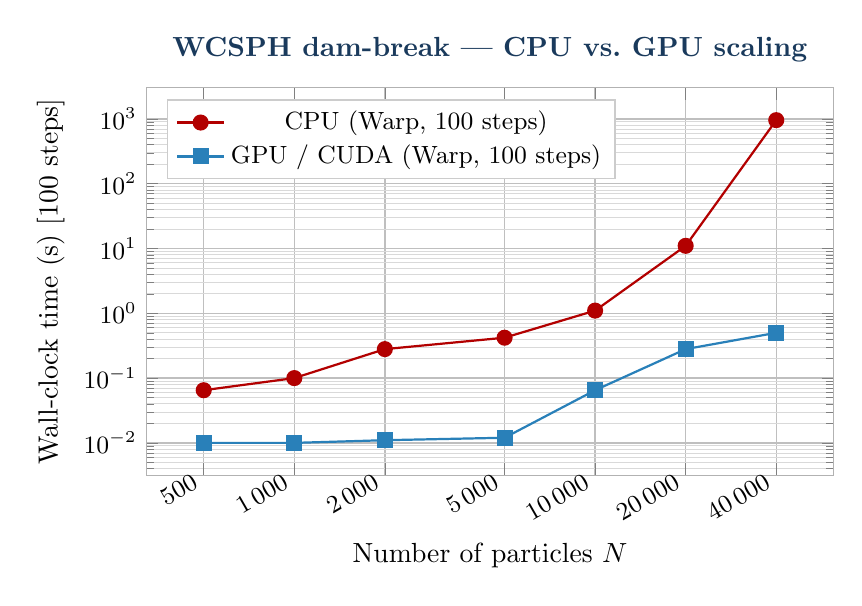
\begin{tikzpicture}
\begin{loglogaxis}[
  width=0.85\linewidth, height=6.5cm,
  xlabel={Number of particles $N$},
  ylabel={Wall-clock time (s) [100 steps]},
  title={\textbf{WCSPH dam-break — CPU vs.\ GPU scaling}},
  grid=both,
  grid style={line width=0.3pt, draw=gray!30},
  major grid style={line width=0.5pt, draw=gray!50},
  legend pos=north west,
  legend style={font=\small, fill=white, draw=gray!40},
  xtick={500,1000,2000,5000,10000,20000,40000},
  xticklabels={500,1\,000,2\,000,5\,000,10\,000,20\,000,40\,000},
  x tick label style={rotate=30, anchor=east, font=\small},
  y tick label style={font=\small},
  tick label style={font=\small},
  title style={color=primary},
  axis line style={color=gray!60},
]
% CPU data (Warp, 100 steps)
\addplot[color=red!70!black, mark=*, thick, mark size=2.5pt] coordinates {
  (500,   0.065)
  (1000,  0.10)
  (2000,  0.28)
  (5000,  0.42)
  (10000, 1.1)
  (20000, 11.0)
  (40000, 957.0)
};
\addlegendentry{CPU (Warp, 100 steps)}

% GPU / CUDA data
\addplot[color=accent, mark=square*, thick, mark size=2.5pt] coordinates {
  (500,   0.010)
  (1000,  0.010)
  (2000,  0.011)
  (5000,  0.012)
  (10000, 0.065)
  (20000, 0.28)
  (40000, 0.50)
};
\addlegendentry{GPU / CUDA (Warp, 100 steps)}
\end{loglogaxis}
\end{tikzpicture}
\end{center}

\vspace{4pt}

The GPU advantage widens with $N$ consistent with $O(N^2)$ CPU vs.\ $O(N)$ GPU scaling;
the full speedup table across all particle counts appears in the Performance Analysis section.
 \newpage
% ── 4  Code Design ───────────────────────────────────────────────────────────
\section{Code Architecture \& Optimisation}

\subsection{Module Overview}

\begin{tabularx}{\linewidth}{>{\ttfamily}lX}
  \toprule
  \textbf{Module} & \textbf{Responsibility} \\
  \midrule
  main.py          & Creates \texttt{SPHConfig}, initialises particles, runs simulation,
                     encodes frames to \texttt{dam\_break.mp4} via FFMpeg. \\
  config.py        & \texttt{SPHConfig} dataclass: domain ($L_x{=}20$, $L_y{=}15$),
                     fluid ($\rho_0{=}1000$, $c_0{=}20$, $\gamma{=}7$), spacing
                     ($\Delta x$, $h{=}1.6\,\Delta x$), time ($\Delta t{=}10^{-4}$). \\
  initialization.py& Lattice dam: meshgrid in $[0,5]\times[0,10]$, converts to
                     \texttt{wp.array(dtype=wp.vec2)}. \\
  simulation.py    & Timestep loop: build HashGrid $\to$ density $\to$ pressure $\to$
                     acceleration $\to$ RK4 $\to$ enforce boundaries. \\
  density.py       & \texttt{\_density\_neighbors\_kernel}: accumulates
                     $\rho_i = \sum_j m_j\,W(|\mathbf{r}_i - \mathbf{r}_j|, h)$
                     over HashGrid neighbours. \\
  forces.py        & \texttt{\_acceleration\_neighbors\_kernel}: pressure gradient
                     (Tait EOS) + Monaghan 1992 artificial viscosity + gravity. \\
  kernels.py       & Monaghan cubic-spline $W$ and $\nabla W$ as \texttt{@wp.func}. \\
  pressure.py      & Tait EOS: $P_i = B\!\left[(\rho_i/\rho_0)^\gamma - 1\right]$,
                     $B = c_0^2\rho_0/\gamma$. \\
  viscosity.py     & Monaghan artificial viscosity $\Pi_{ij}$. \\
  boundaries.py    & Reflective walls with velocity damping $(\times 0.5)$. \\
  integrator.py    & Fused RK4: 4 stages, each computes and writes $k$ pos/vel
                     in a single kernel; finalise with weighted sum. \\
  neighbors.py     & Wraps \texttt{wp.HashGrid}: packs 2-D pos to 3-D, calls
                     \texttt{grid.build()} each step. \\
  \bottomrule
\end{tabularx}

\subsection{Optimisation Strategies}

\begin{enumerate}[leftmargin=1.5em, itemsep=4pt]

\item \textbf{Warp JIT compilation (\texttt{@wp.kernel} / \texttt{@wp.func}).}
  All physics functions are written in Python-syntax Warp kernels.
  On first call they are compiled to CUDA PTX and cached to disk;
  subsequent timesteps execute native GPU code with zero Python interpreter overhead.

\item \textbf{Device-resident arrays.}
  Positions, velocities, densities, pressures, and accelerations live permanently in
  \texttt{wp.array} objects on the GPU.
  No host–device PCIe transfers occur inside the simulation loop.

\item \textbf{Fused RK4 integrator.}
  Each of the four RK4 stages is a single \texttt{@wp.kernel} that computes the stage
  state \emph{and} writes the next $k$-position in one pass, avoiding a separate copy
  kernel. The finalise kernel accumulates all four slopes
  $\Delta \mathbf{r} = \tfrac{\Delta t}{6}(k_1 + 2k_2 + 2k_3 + k_4)$ in registers.
  This achieves fourth-order time accuracy with minimal extra memory traffic versus
  the leapfrog baseline.

\item \textbf{Deferred batch rendering.}
  Raw particle arrays are snapshotted every 500 steps; MP4 encoding runs after the
  simulation completes.
  This prevents GPU–display synchronisation stalls that would otherwise idle the
  compute pipeline.

\end{enumerate}

\subsection{Bottlenecks \& Future Work}

\begin{enumerate}[leftmargin=1.5em, itemsep=3pt]
  \item \textbf{Memory latency.} SM compute utilisation is 1.85\,\% vs.\ 12.93\,\% DRAM — the GPU stalls waiting on $\sim$21 random neighbour reads per particle. Morton Z-order sorting of particles would improve spatial locality by $\approx$30–50\,\%.
  \item \textbf{Full grid rebuild every step.} \texttt{DeviceRadixSort} runs $O(N\log N)$ each timestep despite most particles moving $<$3\,\% of a cell width ($0.001$\,m vs.\ $2h = 0.032$\,m). An incremental linked-list update would cut this cost by $\approx$70–80\,\%.
  \item \textbf{Low occupancy / tail wave.} At $N = 40\,\text{K}$ only 7\,\% of CUDA cores are active. At $N = 500\,\text{K}$ on the RTX 6000 Blackwell the 0.60 partial tail wave wastes $\sim$10\,\% of capacity; tuning to $N = 385\,024$ or $577\,536$ eliminates it.
  \item \textbf{Single-GPU limit.} Multi-GPU domain decomposition with ghost-particle exchange would give $\sim N_\text{GPU}\times$ linear scaling.
\end{enumerate}
\end{document}
